\documentclass{beamer}

\usetheme[progressbar=frametitle]{Warsaw}
\definecolor{mygreen}{rgb}{.125,.5,.25}
\usecolortheme[named=mygreen]{structure}


\title{A.L.E.C.}
\subtitle{\LARGE {Artificial Linguistic Enquiry Chatbot}}
\author[MCA, MNNIT Allahabad]{\Small{Aishwarya Sadana (2017CA12) \linebreak Aditya Bhawsar(2017CA59) \linebreak Mansi Sharma (2017CA79) \linebreak Pavan Chandravanshi (2017CA56) \linebreak \linebreak Under the supervision of \linebreak Dr. Anoj Kumar}}
\institute{Computer Science and Engineering Department \linebreak MNNIT Allahabad, Prayagraj (U.P.)}

\date{May, 2019}

\begin{document}
\begin{frame}
\titlepage
\end{frame}

\begin{frame}{Content}
\begin{enumerate}
    \item Introduction
    \item Problem Statement
    \item About A.L.E.C.
    \item Natural Language Tool Kit (NLTK)
    \item ChatterBot Python Library
    \item Python's SimpleWebSocketServer
    \item Design 
    \item Implementation
    \item Experimental Results
    \item Conclusion \& Future Aspect
    \item References
\end{enumerate}
    
\end{frame}

\begin{frame}{Introduction}
\begin{itemize}
	\item[$\ast$] What is CHATBOT ?
	\linebreak
    \item[--] a computer program or an artificial intelligence which conducts a conversation via auditory or textual methods.
    \linebreak
    \item[--] Helps to find answers to queries through chat 
    \linebreak
    \item[--] Example : Cortana, Siri, Google Assistant etc.
\end{itemize}
\end{frame}
\begin{frame}{Problem Statement ( Why we need A.L.E.C. ?)}
\begin{itemize}
    \item[--] Hard to find information on website.
    \linebreak
    \item[--] Student needs to visit department office manually.
    \linebreak
    \item[--] Limited information on Website.
    \linebreak
    \item[--] It can consumes lot's of time and money.
    \linebreak
    \item[--] Lack of knowledge about department's event.
\end{itemize}
\end{frame}

\begin{frame}{About A.L.E.C. (Artificial Linguistic Enquiry Chatbot )}

\begin{itemize}
    \item[--] One place solution to all the queries ask by student.
    \linebreak
    \item[--] Attached with department notice board.
    \linebreak
    \item[--] Give information about departments Faculties, Events, Facilities, Exam, Assignment, Current Project and Courses etc.
    \linebreak
    \item[--] It also provides :
      \begin{itemize}
          \item[$\ast$]  Chat View.
          \item[$\ast$]  Active Communication Method.
          \item[$\ast$]  27*7 Assistant.
      \end{itemize}
\end{itemize}
    
\end{frame}

\begin{frame}{NLP (Natural Language Processing)}
Before implementation we need to understand some basic working of any chatbot.
\linebreak
\begin{itemize}
    \item[--] It is the branch of machine learning which is about analyzing any text and handling predictive analysis.
    \linebreak
    \item[--] Natural language processing (NLP) is an area of computer science and artificial intelligence concerned with the interactions between computers and human (natural) languages.
    \linebreak
    \item[--] It uses Natural Language Tool Kit.
    \linebreak
    \item[--] The NLTK is a set of Python modules to carry out many common natural language tasks.
\end{itemize}
    
\end{frame}
\begin{frame}{ChatterBot Python library}
   \begin{itemize}
    \item[--] ChatterBot is a Python library that makes it easy to generate automated responses to a user’s input.    
    \linebreak
    \item[--] ChatterBot uses a selection of machine learning algorithms to produce different types of responses. 
    \linebreak
    \item[--] This makes it easy for developers to create chat bots and automate conversations with users.
   \end{itemize}
\end{frame}

\begin{frame}{SimpleWebSocketServer}
 \begin{itemize}
     \item A python based websocket server.
     \linebreak
     \item Asynchronous WebSocket handler
     \linebreak
     \item It uses 3 methods.
     \linebreak
     \begin{itemize}
         \item[$\ast$] handelMessage().
         \linebreak
         \item[$\ast$] handelConnected().
         \linebreak
         \item[$\ast$] handelClose().
     \end{itemize}
 \end{itemize}
    
\end{frame}

\begin{frame}{Design}
    \begin{itemize}
        \item[--] Data Flow Diagram of A.L.E.C.
        \linebreak
        \item[$\ast$] Level 0 :
        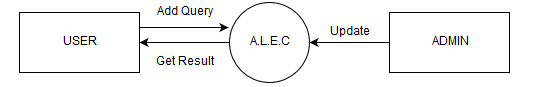
\includegraphics[width=11cm, height=3cm]{Level1_DFD.PNG}
    \end{itemize}
\end{frame}

\begin{frame}{Design}
   \begin{itemize}
       \item[$\ast$] Level 1 :
        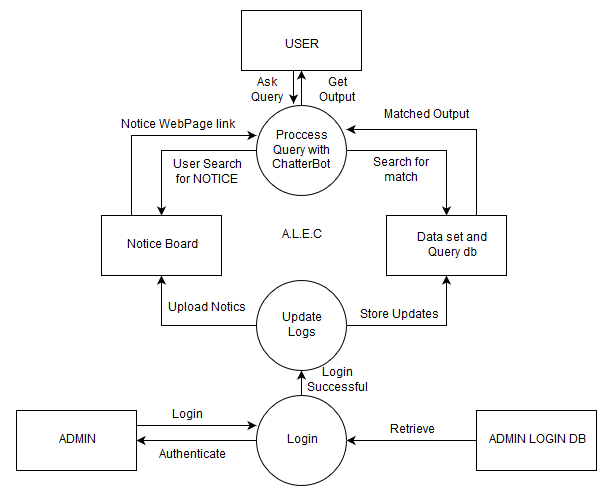
\includegraphics[width=11cm, height=7.5cm]{Level2_DFD.PNG}      
   \end{itemize}
    
\end{frame}

\begin{frame}{Implementation}
A.L.E.C consist of 3 modules :
\linebreak
    \begin{enumerate}
        \item User.
          \begin{itemize}
              \item[--] Ask Query.
              \item[--] Submit New Query.
              \item[--] View Notice Board.
          \end{itemize}
        \item Admin.
           \begin{itemize}
               \item[--] Update/Delete information.
               \item[--] Upload/Delete Notice.   
               \item[--] Register user to upload notice.
           \end{itemize}
        \item Notice.
          \begin{itemize}
              \item[--] This module is defined for displaying the important notices issued by the department. Students can view the notice board by just typing ‘Notice’ in the chatbot. 
          \end{itemize}
    \end{enumerate}
        
\end{frame}

\begin{frame}{Implementation}
  \begin{itemize}
      \item \Large{Corpus Data sets.}
      \linebreak
        \begin{itemize}
            \item[--]  Corpus is a large collection of texts. It is a body of written or spoken material upon which alinguistic analysis is based. A.L.E.C uses text files with .yml (extension) text files for data sets. Like,
            \linebreak
            \linebreak
             - - What is full form of MCA ?
            \linebreak
             - Master of Computer Application
             \linebreak
             - - Number of seats in MCA.
             \linebreak
             - 93 seats.
             \linebreak
             - - How many faculties are under CSED?
             \linebreak
             - There are 21 faculties.
             \linebreak
             - - Subjects taught by Neeraj Tyagi Sir in UG Courses.
             \linebreak
  - Computer Network, Unix Shell Programming etc.
        \end{itemize}
  \end{itemize}
    
\end{frame}
\begin{frame}{Languages Used}
       \begin{itemize}
           \item[--] For Back-End
           \linebreak
           \begin{enumerate}
               \item Python
               \linebreak
               \item PHP
               \linebreak
               \item MySQL
               \linebreak
           \end{enumerate}
           
           \item[--] For Front-End
           \linebreak
           \begin{enumerate}
               \item HTML
               \linebreak
               \item CSS
               \linebreak
               \item Java Script
           \end{enumerate}
       \end{itemize}
    
\end{frame}

\begin{frame}{Experimental Results}
   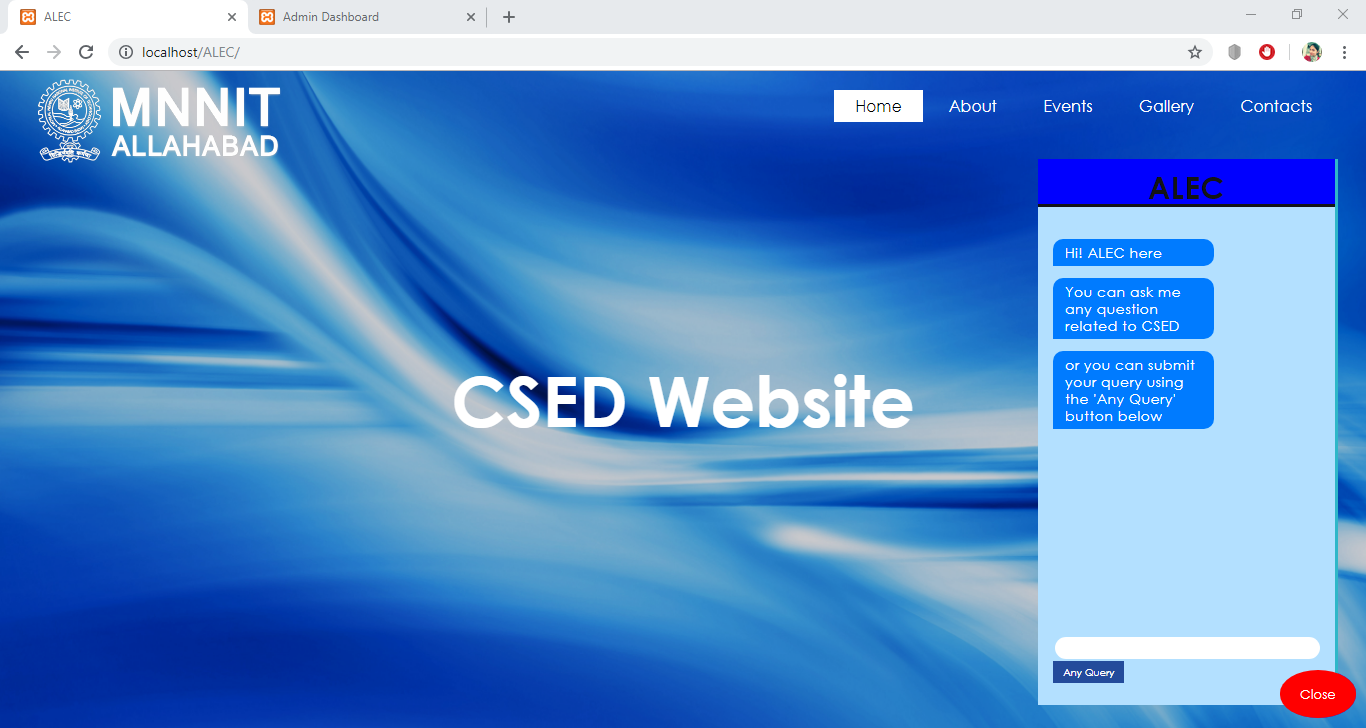
\includegraphics[width=11cm, height=7cm]{s1.png}
   
\end{frame}
\begin{frame}{Experimental Results}
   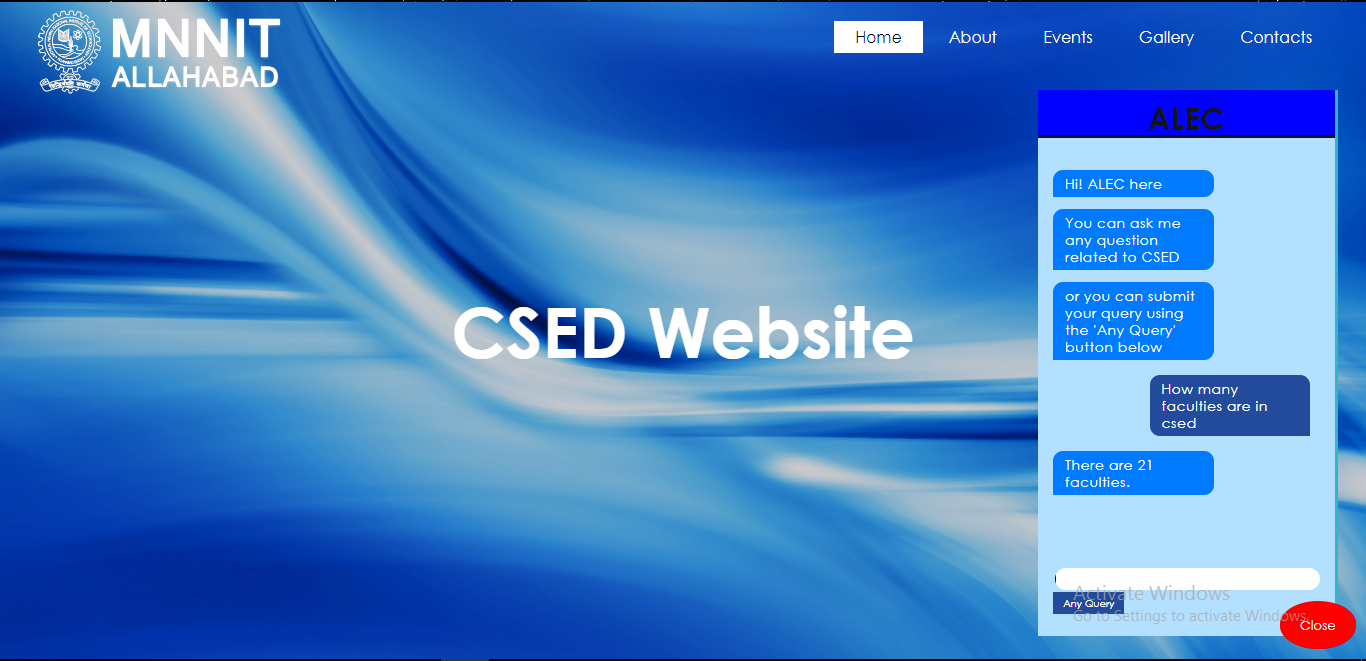
\includegraphics[width=11cm, height=7cm]{s2.PNG}
   
\end{frame}\begin{frame}{Experimental Results}
   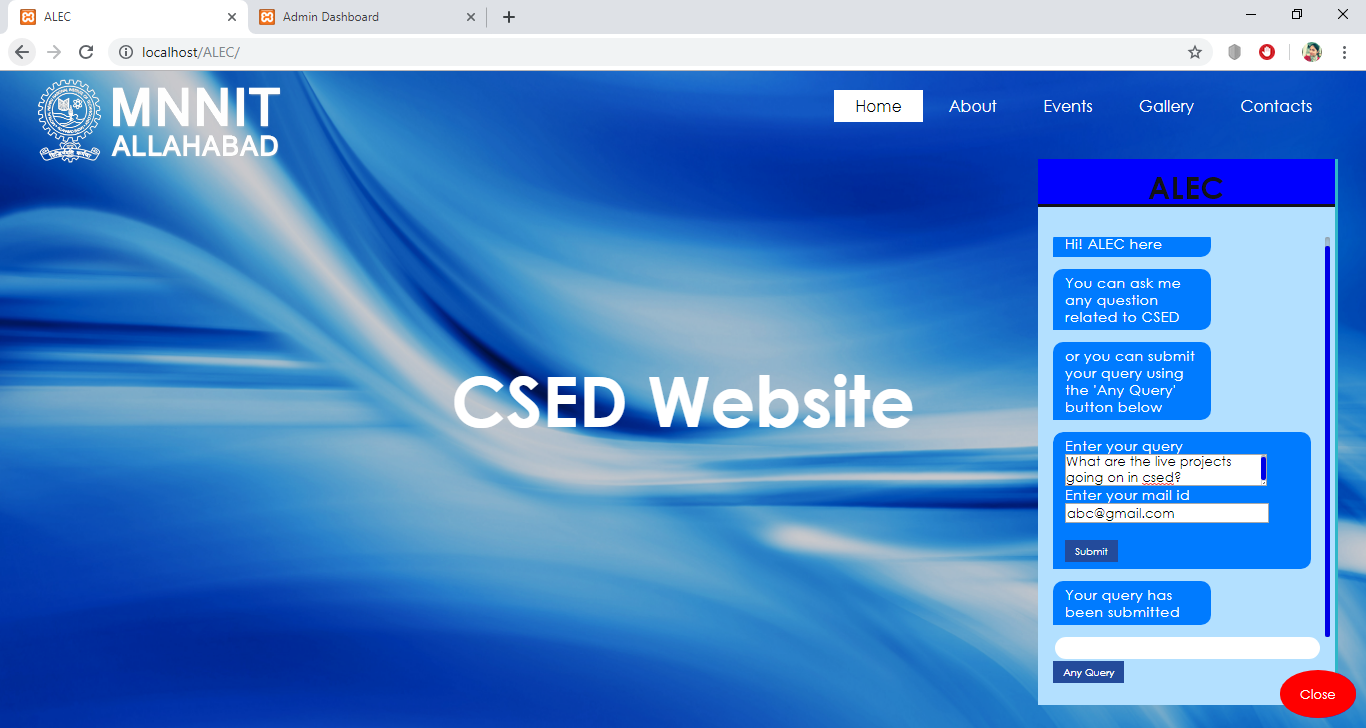
\includegraphics[width=11cm, height=7cm]{s3.png}
   
\end{frame}\begin{frame}{Experimental Results}
   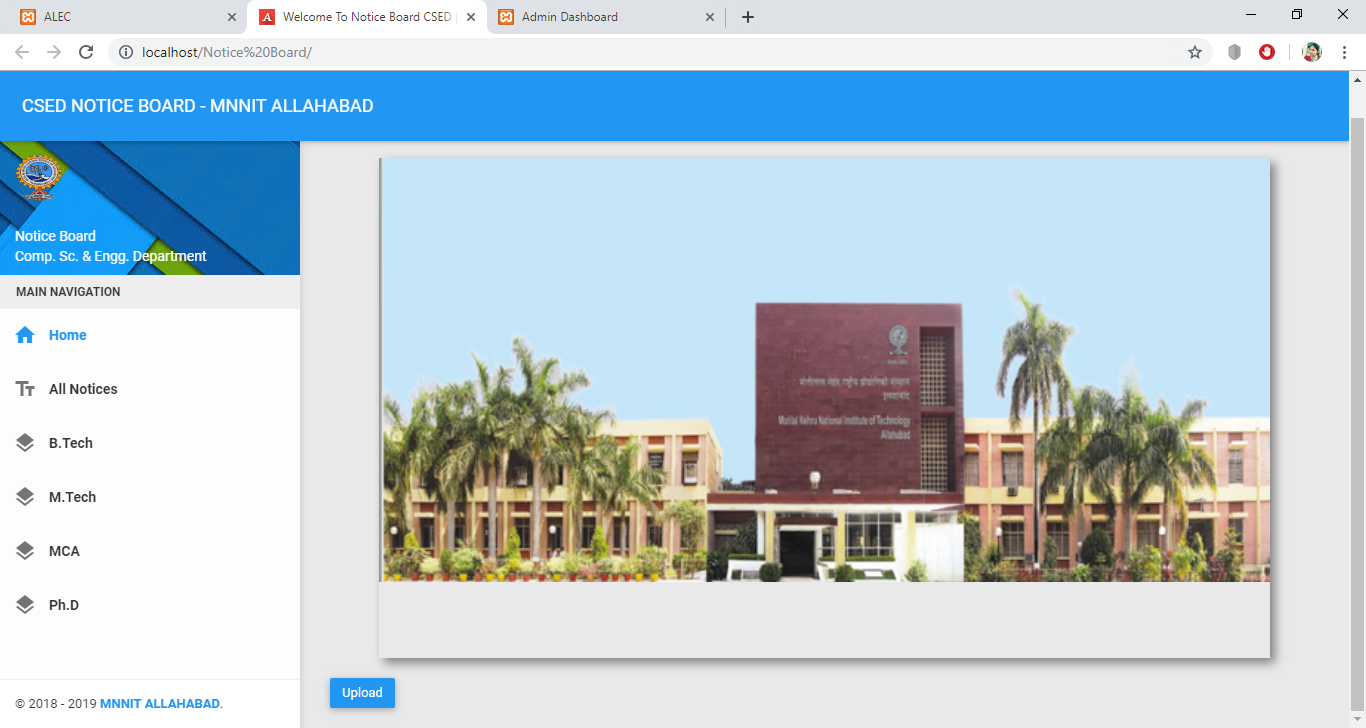
\includegraphics[width=11cm, height=7cm]{s4.png}
   
\end{frame}
\begin{frame}{Experimental Results}
   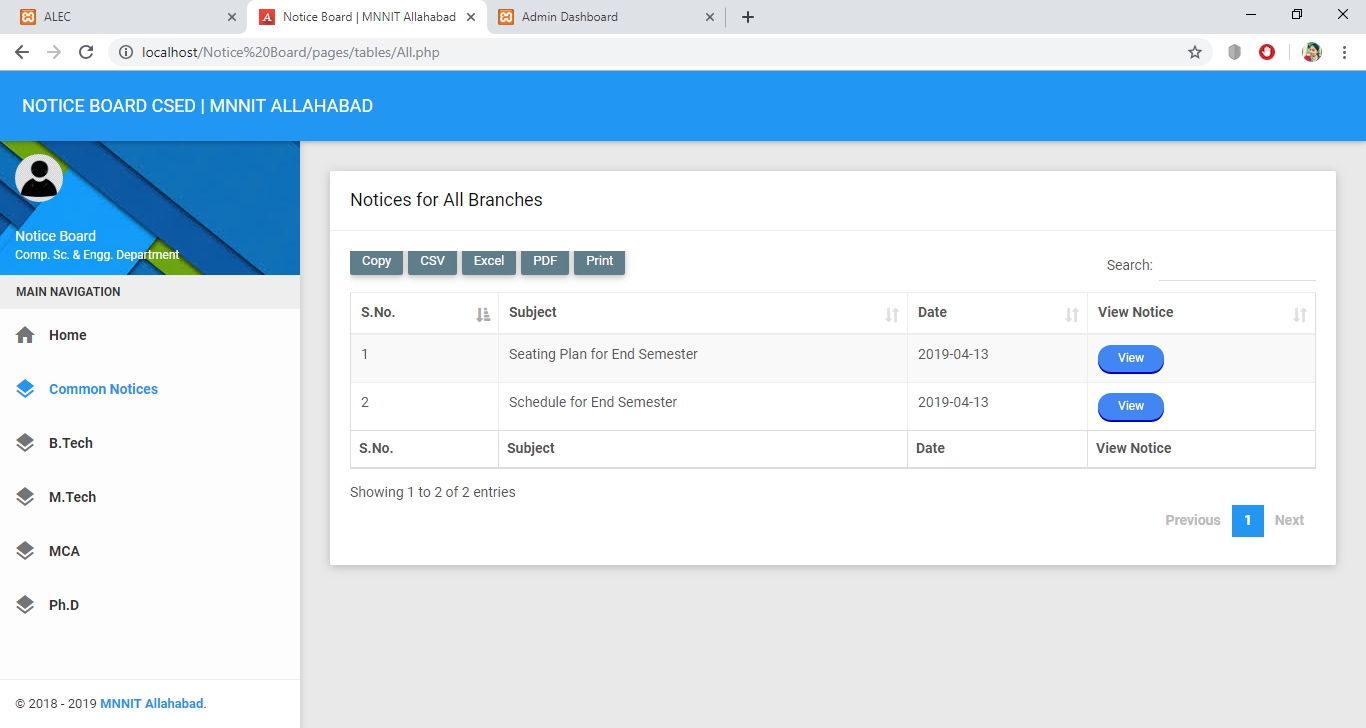
\includegraphics[width=11cm, height=7cm]{s5.png}
   
\end{frame}
\begin{frame}{Conclusion \& Future Aspect}
We now have a Web-app for our CSED Department that will be useful for the students to find answers to their queries. Though it may have a very limited number of features as of now, it can very easily be modified to add new features.
\linebreak
In future many other functionalities can be added to the portal like:
\begin{itemize}
    \item[--] Answers with the available options.
    \item[--] Image and PDF in the answers.
    \item[--] Speech to text and text to speech feature.
    \item[--] User login for more specific queries like assignment, marks or exam information.
    \item[--] Publishing on social media platform like Telegram, Messenger etc.
\end{itemize}
\end{frame}

\begin{frame}{References}
    \begin{enumerate}
        \item 	https://drive.google.com/file/d/0B-tCvLzyt01FYlQ2dVRBWEtTNkE/view
        \item https://www.cleverbot.com/Normaluser friendly chatbot.
        \item https://www.irctc.co.in/nget/Arailway guide on IRCEC website.
        \item https://en.m.wikipedia.org/wiki/XamppXamppserver.
        \item https://chatterbot.readthedocs.io/en/stable/

    \end{enumerate}
     
\end{frame}
\begin{frame}{A.L.E.C}
    \begin{center}
      \LARGE{THANK YOU...}
      
    \end{center}
    
   
\end{frame}

\section{Introduction}

\end{document}
